%\documentclass[prd,twocolumn,aps,psfig,showpacs,nofootinbib,nobibnotes,superscriptaddress,preprintnumbers,times]{revtex4}
%\documentclass[prd,twocolumn,aps,psfig,nofootinbib,nobibnotes,superscriptaddress,preprintnumbers,times]{revtex4-2}
\documentclass[prd,aps,psfig,nofootinbib,nobibnotes,superscriptaddress,preprintnumbers,times]{revtex4-2}\setlength{\topmargin}{-14mm}
\usepackage{graphicx,bm,color,amsmath,amssymb, mathtools,subcaption}
\graphicspath{{./fig/}}
\captionsetup{justification   = RaggedRight,
              singlelinecheck = false}

\usepackage[hidelinks]{hyperref}
\hypersetup{
  colorlinks   = true, %Colours links instead of ugly boxes
  urlcolor     = blue, %Colour for external hyperlinks
  linkcolor    = red, %Colour of internal links
  citecolor    = blue %Colour of citations
}

\def\red{\textcolor{red}}
\def\blue{\textcolor{blue}}

\usepackage{braket,orcidlink}

\usepackage{relsize}

%|||||||||||||||||||||||||||||||||||||||||||||||||||||||||||||||||||
%             Customized Commands
%|||||||||||||||||||||||||||||||||||||||||||||||||||||||||||||||||||
%  mathematical abbreviations
%
%
%
\newcommand{\BoldVec}[1]{\mathchoice%
  {\mbox{\boldmath $\displaystyle     #1$}}%
  {\mbox{\boldmath $\textstyle        #1$}}%
  {\mbox{\boldmath $\scriptstyle      #1$}}%
  {\mbox{\boldmath $\scriptscriptstyle#1$}}%
}
%\newcommand{\BoldVec}[1]{\bm{#1}}}
%
% math debs
\newcommand{\EQ}{\begin{equation}}
\newcommand{\EN}{\end{equation}}
\newcommand{\EQA}{\begin{eqnarray}}
\newcommand{\ENA}{\end{eqnarray}}
\newcommand{\eq}[1]{(\ref{#1})}
\newcommand{\EEq}[1]{Equation~(\ref{#1})}
\newcommand{\Eq}[1]{Eq.~(\ref{#1})}
\newcommand{\Eqs}[2]{Eqs~(\ref{#1}) and~(\ref{#2})}
\newcommand{\EEqs}[2]{Equations~(\ref{#1}) and~(\ref{#2})}
\newcommand{\eqs}[2]{(\ref{#1}) and~(\ref{#2})}
\newcommand{\Eqss}[2]{Eqs~(\ref{#1})--(\ref{#2})}
%\newcommand{\Sec}[1]{\S\,\ref{#1}}
%\newcommand{\Secs}[2]{\S\S\,\ref{#1} and~\ref{#2}}
\newcommand{\Sec}[1]{Sec.~\ref{#1}}
\newcommand{\Secs}[2]{Secs.~\ref{#1} and~\ref{#2}}
\newcommand{\App}[1]{Appendix~\ref{#1}}
\newcommand{\Fig}[1]{Fig.~\ref{#1}}
\newcommand{\FFig}[1]{Figure~\ref{#1}}
\newcommand{\Tab}[1]{Table~\ref{#1}}
\newcommand{\Figs}[2]{Figs.~\ref{#1} and \ref{#2}}
\newcommand{\Tabs}[2]{Tables~\ref{#1} and \ref{#2}}
%\newcommand{\bra}[1]{\langle #1\rangle}
\newcommand{\bbra}[1]{\left\langle #1\right\rangle}
\newcommand{\mean}[1]{\overline #1}
\newcommand{\meanB}{\overline{B}}
\newcommand{\meanC}{\overline{C}}
\newcommand{\meanU}{\overline{U}}
\newcommand{\meanW}{\overline{W}}
\newcommand{\meanPhi}{\overline{\Phi}}
\newcommand{\meanF}{\overline{\cal F}}
\newcommand{\meanR}{\overline{\cal R}}
\newcommand{\meanAA}{\overline{\bm{A}}}
\newcommand{\meanBB}{\overline{\bm{B}}}
\newcommand{\meanEE}{\overline{\bm{E}}}
\newcommand{\meanUU}{\overline{\bm{U}}}
\newcommand{\meanWW}{\overline{\bm{W}}}
\newcommand{\meanJJ}{\overline{\mbox{\boldmath $J$}}}
\newcommand{\meanuu}{\overline{\mbox{\boldmath $u$}}}
\newcommand{\meanGG}{\overline{\mbox{\boldmath $G$}}}
\newcommand{\meanAB}{\overline{\mbox{\boldmath $A\cdot B$}}}
\newcommand{\meanAoBo}{\overline{\mbox{\boldmath $A_0\cdot B_0$}}}
\newcommand{\meanApoBpo}{\overline{\mbox{\boldmath $A'_0\cdot B'_0$}}}
\newcommand{\meanApBp}{\overline{\mbox{\boldmath $A'\cdot B'$}}}
\newcommand{\meanuxB}{\overline{\mbox{\boldmath $\delta u\times \delta B$}}}
\newcommand{\meanemfs}{\overline{\cal E} {}}
\newcommand{\meanemf}{\overline{\mbox{\boldmath ${\cal E}$}} {}} %redundant
\newcommand{\meanAAAA}{\overline{\mbox{\boldmath ${\mathsf A}$}} {}}
\newcommand{\meanSSSS}{\overline{\mbox{\boldmath ${\mathsf S}$}} {}}
\newcommand{\meanAAA}{\overline{\mathsf{A}}}
\newcommand{\meanSSS}{\overline{\mathsf{S}}}
\newcommand{\meanCC}{\overline{\mbox{\boldmath ${\cal C}$}} {}}
\newcommand{\meanFF}{\overline{\mbox{\boldmath ${\cal F}$}} {}}
\newcommand{\meanRR}{\overline{\mbox{\boldmath ${\cal R}$}} {}}
\newcommand{\calFF}{\overline{\mbox{\boldmath ${\cal F}$}} {}}
\newcommand{\meanEMF}{\overline{\mbox{\boldmath ${\cal E}$}} {}}
\newcommand{\tildeFFFF}{\tilde{\mbox{\boldmath ${\cal F}$}}{}}{}
\newcommand{\hatFFFF}{\hat{\mbox{\boldmath ${\cal F}$}}{}}{}
\newcommand{\meanFFFF}{\overline{\mbox{\boldmath ${\cal F}$}}{}}{}
\newcommand{\meanFFF}{\overline{\cal F}}
\newcommand{\hatOO}{\hat{\bm{\Omega}}}
\newcommand{\hatAA}{\hat{\bm{A}}}
\newcommand{\hatBB}{\hat{\bm{B}}}
\newcommand{\tildeh}{\tilde{h}}
\newcommand{\tildeT}{\tilde{T}}
\newcommand{\tildehhh}{\tilde{\sf h}}
\newcommand{\tildeTTT}{\tilde{\sf T}}
%
% tilde
%
\newcommand{\eee}{{\sf e}}
\newcommand{\hhh}{{\sf h}}
\newcommand{\TTT}{{\sf T}}
\newcommand{\tildexx}{\tilde{\bm{x}}}
\newcommand{\tildeBB}{\tilde{\bm{B}}}
\newcommand{\tildeJJ}{\tilde{\bm{J}}}
\newcommand{\tildeA}{\tilde{A}}
\newcommand{\tildeB}{\tilde{B}}
\newcommand{\tildeJ}{\tilde{J}}
\newcommand{\tildeemf}{\tilde{\cal E}}
\newcommand{\teps}{\tilde{\epsilon} {}}
\newcommand{\tkapz}{\tilde{\kappa_0}}
\newcommand{\Oh}{\hat{\Omega}}
\newcommand{\zh}{\hat{z}}
\newcommand{\PC}{{\sc Pencil Code}~}
\newcommand{\PCS}{{\sc Pencil Code}}
%
%  unit vectors
%
\newcommand{\nullvector}{{\bf0}}
\newcommand{\nnn}{\hat{\mbox{\boldmath $n$}} {}}
\newcommand{\vvv}{\hat{\mbox{\boldmath $v$}} {}}
\newcommand{\rr}{\hat{\mbox{\boldmath $r$}} {}}
\newcommand{\xxx}{\hat{\mbox{\boldmath $x$}} {}}
\newcommand{\yyy}{\hat{\mbox{\boldmath $y$}} {}}
\newcommand{\zz}{\hat{\mbox{\boldmath $z$}} {}}
\newcommand{\pp}{\hat{\mbox{\boldmath $\phi$}} {}}
\newcommand{\ttt}{\hat{\mbox{\boldmath $\theta$}} {}}
\newcommand{\OOO}{\hat{\mbox{\boldmath $\Omega$}} {}}
\newcommand{\ooo}{\hat{\mbox{\boldmath $\omega$}} {}}
\newcommand{\BBBB}{\hat{\mbox{\boldmath $B$}} {}}
\newcommand{\kunit}{\hat{\mbox{$k$}} {}}
\newcommand{\nunit}{\hat{\mbox{$n$}} {}}
%
%  hatted quantities
%
\newcommand{\hatU}{\hat{U}}
\newcommand{\hatUU}{\hat{\bm{U}}}
%
%  vectors
%
\newcommand{\gggg}{\BoldVec{g} {}}
\newcommand{\ddd}{\BoldVec{d} {}}
\newcommand{\rrr}{\BoldVec{r} {}}
\newcommand{\xx}{\BoldVec{x}{}}
\newcommand{\yy}{\BoldVec{y} {}}
\newcommand{\zzz}{\BoldVec{z} {}}
\newcommand{\uu}{\BoldVec{u} {}}
\newcommand{\vv}{\BoldVec{v} {}}
\newcommand{\ww}{\BoldVec{w} {}}
\newcommand{\mm}{\BoldVec{m} {}}
\newcommand{\PP}{\BoldVec{P} {}}
\newcommand{\QQ}{\BoldVec{Q} {}}
\newcommand{\RR}{\BoldVec{R} {}}
\newcommand{\UU}{\BoldVec{U} {}}
\newcommand{\bb}{\BoldVec{b} {}}
\newcommand{\qq}{\BoldVec{q} {}}
\newcommand{\BB}{\BoldVec{B} {}}
\newcommand{\HH}{\BoldVec{H} {}}
\newcommand{\II}{\BoldVec{I} {}}
\newcommand{\AAA}{\BoldVec{A} {}}
\newcommand{\aaa}{\BoldVec{a} {}}
\newcommand{\aaaa}{\BoldVec{a} {}} %(convert aaa -> aaaa, compatibility problem)
%\newcommand{\eee}{\BoldVec{e} {}}
\newcommand{\jj}{\BoldVec{j} {}}
\newcommand{\JJ}{\BoldVec{J} {}}
\newcommand{\nn}{\BoldVec{n} {}}
\newcommand{\ee}{\BoldVec{e} {}}
\newcommand{\ff}{\BoldVec{f} {}}
\newcommand{\hh}{\BoldVec{h} {}}
\newcommand{\EE}{\BoldVec{E} {}}
\newcommand{\FF}{\BoldVec{F} {}}
\newcommand{\TT}{\BoldVec{T} {}}
\newcommand{\CC}{\BoldVec{C} {}}
\newcommand{\KK}{\BoldVec{K} {}}
\newcommand{\MM}{\BoldVec{M} {}}
\newcommand{\GG}{\BoldVec{G} {}}
\newcommand{\kk}{\BoldVec{k} {}}
\newcommand{\SSS}{\BoldVec{S} {}}
\newcommand{\grav}{\BoldVec{g} {}}
\newcommand{\nab}{\BoldVec{\nabla} {}}
\newcommand{\OO}{\BoldVec{\Omega} {}}
\newcommand{\oo}{\BoldVec{\omega} {}}
\newcommand{\LL}{\BoldVec{\Lambda} {}}
\newcommand{\llambda}{\BoldVec{\lambda} {}}
\newcommand{\pomega}{\BoldVec{\varpi} {}}
%
%  correlation tensors
%
\newcommand{\RRRR}{\bm{\mathsf{R}}}
\newcommand{\SSSS}{\bm{\mathsf{S}}}
\newcommand{\LLLL}{\mbox{\boldmath ${\sf L}$} {}}
\newcommand{\MMMM}{\bm{\mathsf{M}}}
\newcommand{\BBB}{\mbox{\boldmath ${\cal B}$} {}}
\newcommand{\emf}{\mbox{\boldmath ${\cal E}$} {}}
\newcommand{\FFF}{\mbox{\boldmath ${\cal F}$} {}}
\newcommand{\GGG}{\mbox{\boldmath ${\cal G}$} {}}
\newcommand{\HHH}{\mbox{\boldmath ${\cal H}$} {}}
\newcommand{\QQQ}{\mbox{\boldmath ${\cal Q}$} {}}
%
%  operators  (roman)
%
\newcommand{\ii}{{\rm i}}
\newcommand{\grad}{{\rm grad} \, {}}
\newcommand{\curl}{{\rm curl} \, {}}
\newcommand{\dive}{{\rm div}  \, {}}
\newcommand{\Dive}{{\rm Div}  \, {}}
\newcommand{\diag}{{\rm diag}  \, {}}
\newcommand{\DD}{{\rm D} {}}
\newcommand{\dd}{{\rm d} {}}
\newcommand{\const}{{\rm const}  {}}
\newcommand{\crit}{{\rm crit}  {}}
\def\degr{\hbox{$^\circ$}}
\def\la{\mathrel{\mathchoice {\vcenter{\offinterlineskip\halign{\hfil
$\displaystyle##$\hfil\cr<\cr\sim\cr}}}
{\vcenter{\offinterlineskip\halign{\hfil$\textstyle##$\hfil\cr<\cr\sim\cr}}}
{\vcenter{\offinterlineskip\halign{\hfil$\scriptstyle##$\hfil\cr<\cr\sim\cr}}}
{\vcenter{\offinterlineskip\halign{\hfil$\scriptscriptstyle##$\hfil\cr<\cr\sim\cr}}}}}
\def\ga{\mathrel{\mathchoice {\vcenter{\offinterlineskip\halign{\hfil
$\displaystyle##$\hfil\cr>\cr\sim\cr}}}
{\vcenter{\offinterlineskip\halign{\hfil$\textstyle##$\hfil\cr>\cr\sim\cr}}}
{\vcenter{\offinterlineskip\halign{\hfil$\scriptstyle##$\hfil\cr>\cr\sim\cr}}}
{\vcenter{\offinterlineskip\halign{\hfil$\scriptscriptstyle##$\hfil\cr>\cr\sim\cr}}}}}
%
%  numbers
%
\def\Ta{\mbox{\rm Ta}}
\def\Ra{\mbox{\rm Ra}}
\def\Ma{\mbox{\rm Ma}}
\def\Sh{\mbox{\rm Sh}}
\def\Roo{\mbox{\rm Ro}^{-1}}
\def\Pra{\mbox{\rm Pr}}
\def\Pran{\mbox{\rm Pr}}
\def\Pm{\mbox{\rm Pr}_{\rm M}}
\def\Rm{\mbox{\rm Re}_{\rm M}}
\def\Rey{\mbox{\rm Re}}
\def\Imag{\mbox{\rm Im}}
\def\Pe{\mbox{\rm Pe}}
\def\epsK{\epsilon_{\rm K}}
\def\epsM{\epsilon_{\rm M}}
\def\EEi{{\cal E}_i}
\def\EEK{{\cal E}_{\rm K}}
\def\EEM{{\cal E}_{\rm M}}
\def\EEKM{{\cal E}_{\rm K/M}}
\def\EEGW{{\cal E}_{\rm GW}}
\def\OmK{{\Omega}_{\rm K}}
\def\OmM{{\Omega}_{\rm M}}
\def\OmGW{{\Omega}_{\rm GW}}
\def\hrms{{h}_{\rm rms}}
\def\EEtot{{\cal E}_{\rm tot}}
\def\EErad{{\cal E}_{\rm rad}}
\def\EElam{{\cal E}_\lambda}
\def\EEcrit{{\cal E}_{\rm crit}}
\def\HHGW{{\cal H}_{\rm GW}}
\def\HHK{{\cal H}_{\rm K}}
\def\HHM{{\cal H}_{\rm M}}
\def\EGW{E_{\rm GW}}
\def\HGW{H_{\rm GW}}
\def\EK{E_{\rm K}}
\def\EM{E_{\rm M}}
\def\HM{H_{\rm M}}
\def\hc{h_{\rm c}}
\def\cs{c_{\rm s}}
\def\xiM{\xi_{\rm M}}
\def\xiK{\xi_{\rm K}}
\def\kf{k_{\rm f}}
%\def\kf{k_\ast}
\def\vA{v_{\rm A}}
\def\urms{u_{\rm rms}}
\def\Urms{U_{\rm rms}}
\def\Brms{B_{\rm rms}}
\def\kappaOO{\kappa_{\Omega\Omega}}
\def\kappaO{\kappa_{\Omega}}
\def\kappat{\kappa_{\rm t}}
\def\kappatz{\kappa_{\rm t0}}
\def\nut{\nu_{\rm t}}
\def\etatz{\eta_{\rm t0}}
\def\etat{\eta_{\rm t}}
\def\etaT{\eta_{\rm T}}
\def\Beq{B_{\rm eq}}
\def\tmax{t_{\max}}
%
\newcommand{\ea}{{\em et al. }}
\newcommand{\eaa}{{\em et al. }}
\def\half{{\textstyle{1\over2}}}
\def\threehalf{{\textstyle{3\over2}}}
\def\onethird{{\textstyle{1\over3}}}
\def\twothird{{\textstyle{2\over3}}}
\def\fourthird{{\textstyle{4\over3}}}
\def\quarter{{\textstyle{1\over4}}}
%
\newcommand{\W}{\,{\rm W}}
\newcommand{\V}{\,{\rm V}}
\newcommand{\kV}{\,{\rm kV}}
\newcommand{\eV}{\,{\rm eV}}
\newcommand{\MeV}{\,{\rm MeV}}
\newcommand{\GeV}{\,{\rm GeV}}
\newcommand{\T}{\,{\rm T}}
\newcommand{\uG}{\,\mu{\rm G}}
\newcommand{\G}{\,{\rm G}}
\newcommand{\Hz}{\,{\rm Hz}}
\newcommand{\mHz}{\,{\rm mHz}}
\newcommand{\nHz}{\,{\rm nHz}}
\newcommand{\uHz}{\,\mu{\rm Hz}}
\newcommand{\kHz}{\,{\rm kHz}}
\newcommand{\kG}{\,{\rm kG}}
\newcommand{\K}{\,{\rm K}}
\newcommand{\g}{\,{\rm g}}
\newcommand{\s}{\,{\rm s}}
\newcommand{\ms}{\,{\rm ms}}
\newcommand{\cm}{\,{\rm cm}}
\newcommand{\m}{\,{\rm m}}
\newcommand{\km}{\,{\rm km}}
\newcommand{\kms}{\,{\rm km/s}}
\newcommand{\kg}{\,{\rm kg}}
\newcommand{\Mm}{\,{\rm Mm}}
\newcommand{\pc}{\,{\rm pc}}
\newcommand{\kpc}{\,{\rm kpc}}
\newcommand{\Mpc}{\,{\rm Mpc}}
\newcommand{\yr}{\,{\rm yr}}
\newcommand{\Myr}{\,{\rm Myr}}
\newcommand{\Gyr}{\,{\rm Gyr}}
\newcommand{\erg}{\,{\rm erg}}
\newcommand{\mol}{\,{\rm mol}}
\newcommand{\dyn}{\,{\rm dyn}}
\newcommand{\J}{\,{\rm J}}
\newcommand{\RM}{\,{\rm RM}}
\newcommand{\AU}{\,{\rm AU}}
\newcommand{\A}{\,{\rm A}}
%
\def\hX{h_\times}
\def\hT{h_+}
\def\thT{\tilde{h}_+}
\def\thX{\tilde{h}_\times}
\def\dhT{\dot{h}_+}
\def\dhX{\dot{h}_\times}
\def\dhhT{\dot{\hat{h}}_+}
\def\dhhX{\dot{\hat{h}}_\times}
\def\dhhTX{\dot{\hat{h}}_{+/\times}}
\def\dthT{\dot{\tilde{h}}_+}
\def\dthX{\dot{\tilde{h}}_\times}
\def\dthTX{\dot{\tilde{h}}_{+/\times}}
%
%  journals
%
\newcommand{\arXiv}[3]{, ``#3,'' arXiv:#2 (#1).}
\newcommand{\yjcap}[3]{, J.\ Cosmol.\ Astropart.\ Phys. {\bf #2} (#1) #3.}
\newcommand{\yjas}[3]{, J. Atmosph. Sci. {\bf #2}, #3 (#1).}
\newcommand{\yan}[3]{, Astron. Nachr. {\bf #2}, #3 (#1).}
\newcommand{\yact}[3]{, Acta Astron. {\bf #2}, #3 (#1).}
\newcommand{\yana}[3]{, Astron. Astrophys. {\bf #2}, #3 (#1).}
\newcommand{\yanas}[3]{, Astron. Astrophys. Suppl. {\bf #2}, #3 (#1).}
\newcommand{\yanal}[3]{, Astron. Astrophys. Lett. {\bf #2}, #3 (#1).}
\newcommand{\yass}[3]{, Astrophys. Spa. Sci. {\bf #2}, #3 (#1).}
\newcommand{\ysci}[3]{, Science {\bf #2}, #3 (#1).}
\newcommand{\ysph}[3]{, Solar Phys. {\bf #2}, #3 (#1).}
\newcommand{\yjetp}[3]{, Sov. Phys. JETP {\bf #2}, #3 (#1).}
\newcommand{\yspd}[3]{, Sov. Phys. Dokl. {\bf #2}, #3 (#1).}
\newcommand{\ysov}[3]{, Sov. Astron. {\bf #2}, #3 (#1).}
\newcommand{\ysovl}[3]{, Sov. Astron. Lett. {\bf #2}, #3 (#1).}
\newcommand{\ymn}[3]{, Mon.\ Not.\ R.\ Astron.\ Soc.\ {\bf #2}, #3 (#1).}
\newcommand{\ymhd}[3]{, Magnetohydrohydrodyn. {\bf #2}, #3 (#1).}
\newcommand{\yqjras}[3]{, Quart. J. Roy. Astron. Soc. {\bf #2}, #3 (#1).}
\newcommand{\ynat}[3]{, Nature {\bf #2}, #3 (#1).}
\newcommand{\yjfm}[4]{, ``#4,'' J. Fluid Mech. {\bf #2}, #3 (#1).}
\newcommand{\pjfm}[1]{, J. Fluid Mech., in press (#1).}
\newcommand{\sjfm}[1]{, J. Fluid Mech., submitted (#1).}
\newcommand{\ypr}[3]{, Phys.\ Rev.\ {\bf #2}, #3 (#1).}
\newcommand{\yprd}[4]{, ``#4,'' Phys.\ Rev.\ D {\bf #2}, #3 (#1).}
\newcommand{\ypre}[3]{, Phys.\ Rev.\ E {\bf #2}, #3 (#1).}
\newcommand{\yprf}[4]{, ``#4,'' Phys.\ Rev.\ Fluids {\bf #2}, #3 (#1).}
\newcommand{\yprl}[4]{, ``#4,'' Phys.\ Rev.\ Lett.\ {\bf #2}, #3 (#1).}
\newcommand{\yphl}[3]{, Phys.\ Lett.\ {\bf #2}, #3 (#1).}
\newcommand{\pprl}[1]{, Phys. Rev. Lett., in press (#1).}
\newcommand{\yepl}[3]{, Europhys. Lett. {\bf #2}, #3 (#1).}
\newcommand{\pcsf}[2]{, Chaos, Solitons \& Fractals, in press (#1).}
\newcommand{\ycsf}[3]{, Chaos, Solitons \& Fractals{\bf #2}, #3 (#1).}
\newcommand{\yprs}[3]{, Proc. Roy. Soc. Lond. {\bf #2}, #3 (#1).}
\newcommand{\yptrs}[3]{, Phil. Trans. Roy. Soc. {\bf #2}, #3 (#1).}
\newcommand{\yptrsa}[4]{, ``#4,'' Phil. Trans. Roy. Soc. Lond. A, {\bf #2}, #3 (#1).}
\newcommand{\yjcp}[3]{, J. Comp. Phys. {\bf #2}, #3 (#1).}
\newcommand{\yjgr}[3]{, J. Geophys. Res. {\bf #2}, #3 (#1).}
\newcommand{\ygrl}[3]{, Geophys. Res. Lett. {\bf #2}, #3 (#1).}
\newcommand{\yobs}[3]{, Observatory {\bf #2}, #3 (#1).}
\newcommand{\yaj}[3]{, Astronom. J. {\bf #2}, #3 (#1).}
\newcommand{\sapj}[3]{, ``#3,'' Astrophys. J., submitted, arXiv:#2  (#1).}
\newcommand{\papj}[3]{, ``#3,'' Astrophys. J., in press, arXiv:#2  (#1).}
\newcommand{\yapj}[4]{, ``#4,'' Astrophys. J. {\bf #2}, #3 (#1).}
\newcommand{\yapjs}[3]{, Astrophys. J. Suppl. {\bf #2}, #3 (#1).}
\newcommand{\yapjl}[3]{, Astrophys. J. {\bf #2}, #3 (#1).}
\newcommand{\ycqg}[3]{, Class. Quant. Grav. {\bf #2}, #3 (#1).}
\newcommand{\ypp}[3]{, Phys. Plasmas {\bf #2}, #3 (#1).}
\newcommand{\yppcf}[3]{, Plasmas Phys. Contr. Fusion {\bf #2}, #3 (#1).}
\newcommand{\ppp}[1]{, Phys. Plasmas, in press (#1).}
\newcommand{\ypasj}[3]{, Publ. Astron. Soc. Japan {\bf #2}, #3 (#1).}
\newcommand{\ypac}[3]{, Publ. Astron. Soc. Pacific {\bf #2}, #3 (#1).}
\newcommand{\yaraa}[3]{, Ann. Rev. Astron. Astrophys. {\bf #2}, #3 (#1).}
\newcommand{\yanar}[3]{, Astron. Astrophys. Rev. {\bf #2}, #3 (#1).}
\newcommand{\yanp}[3]{, Ann. Phys. {\bf #2}, #3 (#1).}
\newcommand{\yanf}[3]{, Ann. Rev. Fluid Dyn. {\bf #2}, #3 (#1).}
\newcommand{\ypf}[4]{, ``#4,'' Phys. Fluids {\bf #2}, #3 (#1).}
\newcommand{\yphy}[3]{, Physica {\bf #2}, #3 (#1).}
\newcommand{\ygafd}[4]{, ``#4,'' Geophys. Astrophys. Fluid Dyn. {\bf #2}, #3 (#1).}
\newcommand{\yrpp}[3]{, Rep. Prog. Phys. {\bf #2}, #3 (#1).}
\newcommand{\yptp}[3]{, Progr. Theor. Phys. {\bf #2}, #3 (#1).}
\newcommand{\yjour}[5]{, ``#5,'' #2 {\bf #3}, #4 (#1).}
\newcommand{\pjour}[3]{, #2, in press (#1).}
\newcommand{\sjour}[3]{, #2, submitted (#1).}
\newcommand{\yprep}[2]{, #2, preprint (#1).}
\newcommand{\pproc}[3]{, (ed. #3), #2 (#1) (to appear).}
\newcommand{\yproc}[4]{, (ed. #4), pp. #2. #3 (#1).}
\newcommand{\ybook}[3]{, {\em #2}. #3 (#1).}
\newcommand{\neff}{N_{\rm eff}}
\newcommand{\dneff}{\Delta N_{\rm eff}}
\newcommand{\neffv}{N_{\rm eff}^{(\nu)}}

\newcommand{\inv}{\rm inv}

\usepackage{braket}

\begin{document}

\title{Graviton Mass Limits from Gravitational Waves Detection Data and Future Prospects}

\date{\today}
%TK for now the authors are in alphabetical order

\author{Chris~Choi\,\orcidlink{0009-0005-2328-3044}}
\email{Contact author: minyeonc@andrew.cmu.edu}
\affiliation{McWilliams Center for Cosmology and Astrophysics and Department of Physics, \href{https://ror.org/05x2bcf33}{Carnegie Mellon University}, Pittsburgh, Pennsylvania 15213, USA}

\author{Tina~Kahniashvili\,\orcidlink{0000-0003-0217-9852}}
\email{Contact author: tinatin@andrew.cmu.edu}
\affiliation{McWilliams Center for Cosmology and Astrophysics and Department of Physics, \href{https://ror.org/05x2bcf33}{Carnegie Mellon University}, Pittsburgh, Pennsylvania 15213, USA}
\affiliation{School of Natural Sciences and Medicine, \href{https://ror.org/051qn8h41}{Ilia State University}, 0194 Tbilisi, Georgia}
\affiliation{\href{https://ror.org/02gkgrd84}{Abastumani Astrophysical Observatory}, Tbilisi GE-0179, Georgia}


\begin{abstract}
%TK needs to be started with more general form, what is massive gravity? why massive gravity
In general relativity, we expect two polarizations for gravitational waves, corresponding to the tensor plus and cross modes. In massive gravity, three additional modes of polarization arise, corresponding to two vector modes and one scalar mode. We also expect a modification to the dispersion relation for gravitational waves and the angular correlation in pulsar timing arrays due to these five polarization modes. The recent detection of the stochastic gravitational wave background by pulsar timing arrays provides a unique opportunity to explore the possibility of additional polarization modes and thereby constrain massive gravity. We consider the lower bound for graviton-mass constraints from the dispersion relation for future PTA observations and scrutinize the possibility of detection via the effective overlap reduction function. We find that the predicted overlap reduction function for such a graviton mass lies within the standard deviation of the observed angular correlation in the best-case scenario, and in fact better fits the current data according to some PTA observations. Future PTA observation campaigns are therefore able to detect these additional modes of polarization and can be effectively used to constrain the graviton mass. 

\end{abstract}

\maketitle

\section{Introduction}
The standard cosmological concordance model assumes that general relativity (GR) is the correct theory of gravity on cosmological length and time scales, and that the acceleration of the universe
is due to a cosmological constant ($\Lambda$) that has a time-independent energy density and becomes dominant at late times \cite{Copeland:2006wr, Peebles:2002gy}. 
%TK Reference, any recent review
%CC wondering if these papers are recent enough, im guessing probably not
An alternative approach to the late-time accelerated expansion of the universe is
to consider the possibility that the true theory of gravity differs from GR on large scales \cite{Clifton:2011jh, Nojiri:2017ncd, Joyce:2014kja, Planck:2015bue}. 
%TK reference - modified gravity 
%TK commented - rewritten = 
%In the framework of the standard model of cosmology (e.g. concordance model)  and particle physics, the observed accelerated expansion of the Universe today is driven by the substance of unknown nature with a negative pressure (by its modulus equal  to its energy density), the so-called cosmological constant. The requirement of the existence of  the cosmological constant (or any dynamical dark energy) follows from the Einstein equations, which assume  general relativity (GR) as the true theory of gravity, and massless of the graviton, the helicity-2 particles associated with gravitational radiation. 
%Despite the success of the concordance model, there are several unanswered questions, including the hierarchy problem, smallness of gravity compared to the other forces in the standard model, failure to formulate a unified theory of quantum gravity, among many others.  These puzzles suggest that GR is not suitable for describing physical processes at cosmological scales. Many cosmological observables are sensitive to modifications of GR which makes it possible to test GR through current and future planned observations. These tests include the growth of structure in the late time universe, as measured in galaxy surveys; the rate of acceleration of the universe, that can be measured with standard candles and standard rulers; the number density of nonlinear structures, such as clusters that are very sensitive to the strength of gravitational interactions; the temperature and polarization anisotropies of the cosmic microwave background (CMB), and many others. 
%\cite{Jain:2007yk,Jain:2010ka,Jain:2013wgs,Xu:2014uba,Baker:2014zba,Koyama:2015vza,Berti:2015itd,Joyce:2016vqv}.
%%%%%%%%%%%%%%%%%%%%%%%%%%%%%%%%%%%%%%%%%%%%%%%%%%%%%%%%%%%%%%%%%%%%%%%%%%%%%%%%%%%%%%%%%%%%%%%
In addition to providing a theoretical framework that could explain the observed accelerated expansion, modified theories of gravity have a number of other attractive features, such as the possibility to unify late-time acceleration with early inflationary expansion \cite{Hinterbichler:2011tt,Clifton:2011jh,Nojiri:2010wj,Joyce:2014kja} 
and to explain dark matter \cite{Blas:2024jyh, Aoki:2016zgp}. 
If we want to have a unified theory of all interactions, it is quite likely that GR will have to be modified anyway.
%TK Reference
%%%%
One of the most active areas of research in gravity theory stems from the assumption that the graviton has a non-zero mass $m_g$, in a theory known as massive gravity. The idea of a nonzero mass of gravitons (particles responsible for gravitational interactions) has a long history, starting from the formulation of MG at the linear level by Fierz and Pauli \cite{Fierz:1939ix} in the 1930s. In contrast to GR, where gravitational waves have only two degrees of freedom (helicity $\pm 2$, tensor modes), massive gravity theories have an additional three degrees of freedom, namely, the helicity-$0$ (scalar) and helicity $\pm 1$ (vector) modes. As a result, massive gravity theory is subject to the van Dam-Veltman-Zakharov (vDVZ) discontinuity \cite{vanDam:1970vg,Zakharov:1970cc}. That is, in the massless limit as $m_g \rightarrow 0$, the five modes of massive gravity do not reduce to the two modes that we expect in GR, causing, for example, a discrepency in the bending of light around massive objects by a factor of 4/3 \cite{vanDam:1970vg}. Taking into account the non-linear effects of the strong gravitational potential, the Vainshtein mechanism \cite{Vainshtein:1972sx} ensures the screening of additional scalar and vector modes, and correspondingly frees massive gravity from the vDVZ discontinuity\footnote{GR is recovered in a strong gravitational field, allowing us to verify GR in terrestrial and solar system level tests 
%TK reference
}. The effects of massive gravity thus appear only at
cosmological scales, possibly leading to an accelerated expansion.
%TK reference
However, extensions in the nonlinear regime have been found to be unsatisfactory due to the presence of an unhealthy sixth mode \cite{Boulware:1972yco}.\footnote{Until 2010, it was thought that all Lorentz-invariant massive gravity theories were characterized by the unhealthy presence of the ghost-mode, and thus were not valid. }
More recently, groundbreaking progress was made through the formulation of ghost-free massive gravity in the deRham-Gabadadze-Tolley (dRGT) theory \cite{deRham:2010ik,deRham:2010kj}, and its bigravity generalization \cite{Hassan:2011zd}. Since then, different modifications to dRGT and bigravity have been proposed \cite{Hinterbichler:2011tt,deRham:2014zqa,Koyama:2015vza,deRham:2016nuf,Hinterbichler:2016try, Cusin:2016ytz}, leading to investigations into the consequences of massive gravity (massive cosmologies) 
\cite{DAmico:2011eto,Gratia:2012wt,Gumrukcuoglu:2012aa,Maeda:2013bha,Akrami:2013pna,Zhang:2013noa,Lambiase:2012fv,Koyama:2011wx,Tasinato:2012ze,Solomon:2014iwa, Akrami:2013ffa,Koennig:2014ods,Gumrukcuoglu:2016hic}, 
%TK REFERENCES COMPLETE AND UPDATE or keep pioneering, and recent
%TK 
including 
%the stability of solutions (at background and perturbation levels), star and black hole (BH) formation, 
gravitational wave (GW) generation and propagation \cite{DeFelice:2013awa,Gumrukcuoglu:2013nza,DeFelice:2013bxa,DeFelice:2015moy,Babichev:2015xha,Sakstein:2017bws}. 
%TK check references, we need only on GWs
%\cite{Gabadadze:2008ha,deRham:2010tw,Bernard:2014bfa,Comelli:2012db,Wyman:2012iw,Sjors:2011iv,Fasiello:2012rw,DeFelice:2013awa,Gumrukcuoglu:2013nza,DeFelice:2013bxa,Katsuragawa:2015lbl,DeFelice:2015moy,Babichev:2015xha,Li:2016fbf,Sakstein:2017bws},
%
%CC: I have included just the ones regarding GW propogation
%While the theoretical foundation of massive gravity is beyond the scope of the current paper, we aim to place model-independent upper bounds on the graviton mass through gravitational waves observation data and cross-correlate them with limits obtained through different cosmological observations.
%\cite{Gabadadze:2008ha,deRham:2010tw,Bernard:2014bfa,Comelli:2012db,Wyman:2012iw, Sjors:2011iv,Fasiello:2012rw,DeFelice:2013awa, Gumrukcuoglu:2013nza,DeFelice:2013bxa,Katsuragawa:2015lbl DeFelice:2015moy,Babichev:2015xha,Li:2016fbf,Sakstein:2017bws}.
%TK REFERENCES

The following effects of massive gravity on gravitational waves can phenomenologically be used to constrain the graviton mass (see Ref.\ \cite{deRham:2016nuf} for a review):
(i) the presence of a non-zero graviton mass results in a Yukawa-type exponential suppression of the gravitational potential ($\Phi \propto e^{-m_gR}/R$), and correspondingly in suppressing the gravitational waves at wavelength larger than the Compton length scale of the graviton ($R_g \simeq m_g^{-1}$),\footnote{The length scale determined by the graviton mass through the Yukawa suppression can naively be treated as a ``gravitational causal horizon'' and we can expect the correlations of gravitational perturbations to be suppressed outside this ``gravitational causal horizon''.}
(ii) modification of the gravitational wave dispersion relation, as $\omega^2 = k^2 +m_g^2$ (with $\omega$ and $k$ angular frequency and $k$ wavenumber of gravitational waves respectively), i.e. the difference of the gravitational wave propagation speed ($c_g$) from the speed of light ($c$), and
(iii) the additional degrees of polarization (helicity-$0$ and helicity-$\pm 1$). The main consequence of helicity-$0$ polarization for the graviton is a coupling of the helicity-0 mode to matter (the so-called {\it fifth force}) \cite{deRham:2014naa}.\footnote{{However, in dense environments, the Vainshtein mechanism \cite{Vainshtein:1972sx} ensures the screening of the helicity-0 (and helicity-$\pm 1$) mode \cite{deRham:2012fw,
Bloomfield:2014zfa,Falck:2015rsa,Falck:2014jwa,Kase:2015zva,Koyama:2015oma}, while leaving the helicity-$\pm 2$ modes the same as in GR.}}
%TK Rewrite what we do and how
%In this paper, we address the graviton mass limits obtained through their direct detection at high frequencies by the Laser Interferometer Gravitational-Wave Observatory (LIGO) and VIRGO collaborations \cite{LIGOScientific:2016aoc,LIGOScientific:2016sjg}, and at low frequency ranges by the North American Nanohertz Observatory for Gravitational Waves (NANOGrav) collaboration \cite{Agazie:2023}, that has been confirmed by other pulsar timing arrays (PTAs) such as  European PTA (EPTA) \cite{Antoniadis:2023lym,Antoniadis:2023ott}, the Chinese PTA (CPTA) \cite{Xu:2023wog}, and the Parkes Pulsar Timing Array (PPTA) \cite{Zic:2023gta,Reardon:2023gzh}. 

The paper is arranged as follows: in Sec.\ \ref{sec:setup}, we introduce the modified dispersion relation and its consequences. In Sec.\ \ref{sec:overlap}, we derive the modified overlap reduction and discuss frequency-dependence complications. In Sec.\ \ref{sec:results}, we compare the numerical results to the data from NANOGrav 15yr and CPTA. In Sec.\ \ref{sec:discussion}, we discuss the implications of our findings and the potential for further investigations. Throughout this paper, we use  (+,--,--,--) for the Minkowski metric $\eta_{\mu\nu}$, and we use natural units, setting $c = $$\ \hbar = $$\ k_B = $$\ 1$. 


\section{Setup}\label{sec:setup}
In general, the linearized action in massive gravity is given by the Fierz-Pauli action \cite{Fierz:1939ix}, the oldest and simplest of the actions constructed for a massive spin-2 field
\begin{equation}\label{eqn:action}
    \mathcal{S}_{\text{FP}} = \mathcal{S}_{\text{EH}}^{(2)} + S_{\text{m}},
\end{equation}
where we have written it in two parts to explicitly show the mass dependence. Here, $S_{\text{EH}}^{(2)}$ is the quadratic part of the Einstein-Hilbert action and $S_{\text{m}}$ is the massive term
\begin{equation} \label{eqn:action_m}
    S_{\text{m}} = \frac{m_g^2}{2}\int d^4x (h_{\mu\nu}h^{\mu\nu} - h^2),
\end{equation} 
where $m_{g}$ is the mass of the graviton and $h_{\mu\nu}$ is the metric perturbation defined by the metric tensor as follows: $g_{\mu\nu} = \eta_{\mu\nu} + h_{\mu\nu}$. In its original form, the Boulware-Deser ghost is present, so we adopt the ghost-free formulation. Additionally, we use the quadratic expansion because we are only interested in working at the linear level. In order to obtain the equations of motion, in the linear regime, we first take the Fourier transform of the metric perturbation 
\begin{equation}\label{eqn:fourier}
    h_{\mu\nu}(t, {\bf x}) = \int \frac{d^4 k}{(2\pi)}h_{\mu\nu}(t, {\bf k})e^{i{\bf k}\cdot{\bf x}}
\end{equation}
We decompose $h_{\mu\nu}(t, {\bf k}) $ using polarization tensors
\begin{equation}\label{eqn:decomp}
    h_{\mu\nu}(t, {\bf k}) = \sum_{i \in \{\pm 2, \pm 1,0\} } \epsilon^\lambda_{\mu\nu}({\bf k})h^{(i)}(t, {\bf k}),
\end{equation}
where ${\bf k}$ is the wavevector of the graviton and $\epsilon^\lambda_{ij}$ are the polarization tensors given by Table \ref{tbl:tensors} in terms of the massive spin-1 polarization vectors
\begin{equation}\label{eqn:pol_vec}
    \epsilon_\mu^{\pm}(k) = \frac{1}{\sqrt{2}} 
\begin{pmatrix}
0 \\
\cos\theta \cos\varphi \mp i \sin\varphi \\
\cos\theta \sin\varphi \pm i \cos\varphi \\
- \sin\theta
\end{pmatrix}
, \ \ \ \epsilon_\mu^{0}(k) = \frac{1}{\sqrt{k^2}} 
\begin{pmatrix}
|\mathbf{k}| \\
k_0 \sin\theta \cos\varphi \\
k_0 \sin\theta \sin\varphi \\
k_0 \cos\theta
\end{pmatrix} \ .
\end{equation}
Here, $\theta$ and $\varphi$ describe the polar and azimuthal angles that describe the propagating graviton's spatial direction, and $k_0$ is the time-like coordinate of the wavevector, given by $k_0 = 2\pi f$. 
\begin{table}[h] 
\centering
\renewcommand{\arraystretch}{1.8}
\begin{tabular}{|c|c|c|l|}
\hline
\textbf{Mode} & \textbf{Type} & \textbf{Polarization Tensor $e^{\lambda}_{\mu\nu}$} \\
\hline
$\epsilon^{(+2)}_{\mu\nu}$     & Tensor  & $\epsilon^+_\mu \epsilon^+_\nu $ \\
\hline
$\epsilon^{(-2)}_{\mu\nu}$     & Tensor   & $\epsilon^-_\mu \epsilon^-_\nu $ \\
\hline
$\epsilon^{(+1)}_{\mu\nu}$     & Vector   & $\dfrac{1}{\sqrt{2}} \left( \epsilon^+_\mu \epsilon^0_\nu + \epsilon^0_\mu \epsilon^+_\nu \right)$ \\
\hline
$\epsilon^{(-1)}_{\mu\nu}$     & Vector   & $\dfrac{1}{\sqrt{2}} \left( \epsilon^-_\mu \epsilon^0_\nu + \epsilon^0_\mu \epsilon^-_\nu \right)$ \\
\hline
$\epsilon^{(0)}_{\mu\nu}$      & Scalar  & $\dfrac{1}{\sqrt{6}} \left( \epsilon^+_\mu \epsilon^-_\nu + \epsilon^-_\mu \epsilon^+_\nu - 2\epsilon^0_\mu \epsilon^0_\nu \right)$ \\
\hline
\end{tabular}
\caption{Polarization tensors $\epsilon^{(i)}_{\mu\nu}$ of a spin-2 particle expressed in terms of vector polarizations $\epsilon^\lambda_\mu$ for helicities $\lambda = 0, \pm1$.}
\label{tbl:tensors}
\end{table}
We note that this formulation of the polarization tensors is related to the typical set of polarization tensors $\{\epsilon_{\mu\nu}^+, \epsilon_{\mu\nu}^\times, \epsilon_{\mu\nu}^x, \epsilon_{\mu\nu}^y, \epsilon_{\mu\nu}^l \}$ in a nontrivial way \cite{Liang:2021bct}, but it is this formulation that we will use on account of its convenience for describing correlations in pulsars.

We minimize the action from Eq.\ (\ref{eqn:action}) with respect to $h^{(i)}$, and we get the following equation of motion for each polarization mode \cite{Maggiore:v2} 
\begin{equation}\label{eqn:eom}
    \ddot{h}^{(i)}(t, {\bf k}) + 3 H(t)\dot{h}^{(i)}(t, {\bf k}) + \left(\frac{k^2}{a^2(t)} + m_g^2\right)h^{(i)}(t, {\bf k}) = 0 \ ,
\end{equation}
where the dots represent the usual time derivative, $a(t)$ is the scale factor and $H(t)$ is the Hubble parameter. From this, we can easily see that the dispersion relation for the massive graviton is 
\begin{equation}\label{eq:dispersion}
    \omega^2 = \frac{k^2}{a^2} + m_g^2 \ ,
\end{equation}
where $\omega$ is the effective angular frequency, equivalent to $k_0$. Since we are observing gravitational waves at very nearly the present time, we set $a = 1$. Eq.\ \ref{eq:dispersion} provides a lower bound on the frequency for a gravitational wave, given by the mass of the graviton $m_g$, provided that $k$ goes to 0. In other words, $\omega$ must be at least $m_g$. Pulsar-timing arrays are sensitive to frequencies in the range \cite{Moore:2014lga}
\begin{equation}\label{eq:freqrange}
    \frac{1}{T_{\text{obs}}} < f < \frac{1}{\delta t} \ ,
\end{equation} where $T_{\text{obs}}$ is the total length of time the pulsars are observed for and $\delta t$ is the cadence, i.e.\ how often the pulsars are measured. For reference, $T_{\text{obs}} \approx$ 15 years and $\delta t \approx$ 0.5 weeks for the most frequent observations of a pulsar observed in NANOGrav. In section \ref{sec:results}, we discuss how we use Eq.\ \ref{eq:dispersion} in the context of observational prospects. 

\section{Overlap Reduction Functions}\label{sec:overlap}
\subsection{Derivation}\label{subsec:derivation}
Suppose there is a massive gravitational wave propagating in an arbitrary spatial direction specified by the unit vector
\begin{equation}\label{eqn:omega}
    \hat{\Omega} = \begin{pmatrix}
                        \sin\theta \cos\varphi \\
                        \sin\theta \sin\varphi \\
                        \cos\theta
                    \end{pmatrix} \ .
\end{equation}
This gravitational wave affects the pulsar timing measurements by causing pulsar signals, originally emitted with a constant frequency $\nu_0$, to be perturbed as they travel from their source pulsars to our telescopes. 
%Such a wealth of literature has been produced in hopes of capturing   
In the solar system barycenter reference frame, the frequency shift is characterized by the redshift
\begin{equation}\label{eqn:z}
    z(t) = \frac{\nu_0 - \nu(t)}{\nu_0} \ .
\end{equation}
PTA collaborations actually measure the integral of $z(t)$, otherwise known as the anomalous residual, but it is trivial to rewrite these equations in terms of the residual if we so desire. We take advantage of the freedom of choice granted by their simple relation, and we proceed in our analysis using the redshift. Assume we have an electromagnetic wave traveling along a null geodesic 
\begin{equation}\label{eqn:null}
    \sigma^\mu = s^\mu - \frac{1}{2} \eta^{\mu\nu}h_{\nu \gamma}s^\gamma \ .
\end{equation}
Here, $s^\mu \equiv \nu (1, -\hat{\bf p})$ where $\hat{p}$ is the unit vector pointing in the direction of the pulsar from the solar system barycenter, and $h_{\nu \gamma}$ is position dependent, as defined in Eq.\ \ref{eqn:fourier}. This null geodesic obeys the corresponding geodesic equation 
\begin{equation}\label{eqn:geodesic}
    \frac{d\sigma^\mu}{d\lambda} = -\Gamma_{\alpha \beta}^\mu \sigma^\alpha \sigma^\beta \ ,
\end{equation} where $\lambda$ is the affine parameter that describes the null path the electromagnetic signal takes, and $\Gamma_{\alpha \beta}^\mu$ is the Christoffel symbol. After fully expanding the Christoffel symbol and applying the metric tensor, the geodesic equation becomes  
\begin{equation}\label{eqn:geodesic_further}
    \frac{d\sigma^\mu}{d\lambda} = \frac{1}{2}\dot{h}_{\alpha \beta} s^\alpha s^\beta - h_{0\alpha, \beta} s^\alpha s^\beta \ .
\end{equation}
We neglect higher-order terms past the linear order. We now assume that the gravitational wave is propagating as a plane wave, whose metric perturbation takes the following form 
\begin{equation}\label{eqn:plane_wave}
    h_{\mu \nu}(t, \hat{\bf x}) = \int_{-\infty}^\infty df \int d^2 \hat{\bf \Omega} e^{i2\pi f \left(t - \frac{|{\bf k}|}{k_0} \hat{\bf \Omega}\cdot {\bf x}\right)}h_{\mu \nu}\left(f, \frac{|{\bf k}|}{k_0} \hat{\bf \Omega} \right) \ ,
\end{equation}
where ${\bf x}$ is the position vector of the pulsar, $L\hat{\bf p}$. We apply the chain rule on the metric perturbation, and we get
\begin{equation}\label{eqn:dhdlambda}
    \begin{aligned}
        \frac{dh^{(i)}_{\mu \nu} \left(t - \frac{|{\bf k}|}{k_0} \hat{\bf \Omega}\cdot {\bf x}\right) }{d\lambda } &= \frac{\partial h^{(i)}_{\mu \nu}\left(t - \frac{|{\bf k}|}{k_0} \hat{\bf \Omega}\cdot {\bf x}\right) }{\partial t} \frac{dt}{d \lambda} + \frac{\partial h^{(i)}_{\mu \nu}\left(t - \frac{|{\bf k}|}{k_0} \hat{\bf \Omega}\cdot {\bf x}\right) }{\partial (\hat{\bf \Omega}\cdot {\bf x})} \frac{d(\hat{\bf \Omega}\cdot {\bf x})}{d \lambda} \\ &= \nu\left( 1 + \frac{|{\bf k}|}{k_0} \hat{\bf \Omega}\cdot \hat{\bf p}\right) \frac{\partial h^{(i)}_{\mu \nu}\left(t - \frac{|{\bf k}|}{k_0} \hat{\bf \Omega}\cdot {\bf x}\right) }{\partial t} \ .
    \end{aligned}
\end{equation}
Here, we have used Eq.\ \ref{eqn:null} and the intrinsic dependence of the metric perturbation on time and $\hat{\bf \Omega}\cdot {\bf x}$. We now use Eq.\ \ref{eqn:geodesic_further} to get 
\begin{equation}\label{eqn:dnudl}
    \frac{d\nu}{d\lambda} = \nu \left( \frac{1}{2} \frac{\hat{p}^\alpha \hat{p}^\beta}{1+\frac{|\boldsymbol{k}|}{k_0} \hat{\boldsymbol{\Omega}} \cdot \hat{\boldsymbol{p}}}\frac{d h_{\alpha \beta}\left(t - \frac{|\boldsymbol{k}|}{k_0} \hat{\boldsymbol{\Omega}} \cdot {\boldsymbol{x}}\right)}{d \lambda} - \frac{1}{2} \frac{dh_{0\alpha}\left(t - \frac{|\boldsymbol{k}|}{k_0} \hat{\boldsymbol{\Omega}} \cdot {\boldsymbol{x}}\right)}{d\lambda}\hat{p}^\alpha \right) \ .
\end{equation}
This is simply a separable differential equation, and is integrated from some $j$-th pulsar to the solar system barycenter to yield the redshift (which we express in the Fourier space)
\begin{equation}\label{eqn:redshift}
    z(t, \hat{\bf \Omega}) = \int_{-\infty}^\infty df \mathcal{E}_j(f, \hat{\Omega}) \sum_i h^{(i)}\left(f, \frac{|{\bf k}|}{k_0} \hat{\bf \Omega}\right)F^{(i)}_j(\hat{\bf \Omega}) \ ,
\end{equation}
where we have defined the recieving function $F^{(i)}_j(\hat{\bf \Omega}) $ as 
\begin{equation}\label{eqn:recieving}
    F^{(i)}_j(\hat{\Omega}) = \frac{\hat{p}^\mu_j}{2}\left(-\frac{\hat{p}^\nu_j}{1+\frac{|\boldsymbol{k}|}{k_0} \hat{\boldsymbol{\Omega}} \cdot \hat{\boldsymbol{p}_j}} \epsilon_{\mu \nu}^{(i)}+\epsilon_{0 \mu}^{(i)}\right) \ ,
\end{equation}
and the exponential factor $\mathcal{E}_j(f, \hat{\Omega})$ encoding the dependence on the metric perturbation
\begin{equation}
    \mathcal{E}_j(f, \hat{\Omega}) = e^{-i2\pi f L_j\left( 1 + \frac{|{\bf k}|}{k_0} \hat{\bf \Omega}\cdot \hat{\bf p}_j\right)} - 1 \ . 
\end{equation}
We discuss the nature of this exponential factor in more detail in Sec.\ \ref{subsec:exp_fac}. A few details of this derivation have been excluded in this discussion, however, more careful derivations can be found in Refs.\ \cite{Anholm:2008wy, Liang:2021bct}, which ultimately derive from even earlier work \cite{Detweiler:1979wn, Estabrook:1975jtn, Kaufmann:1970}.
For PTA data, a quantity of interest is the two-point correlation of the total redshift, $\langle \tilde{z}(f) \tilde{z}(f') \rangle$, where $\tilde{z}(f)$ is the sky-averaged redshift $\tilde{z}(f) \equiv \int d^2\hat{\bf \Omega} z(f, \hat{\bf \Omega})$. Combining everything we have derived up until now, our expression for the two-point correlation is as follows
\begin{equation}\label{eqn:two_point_z}
    \langle \tilde{z}(f) \tilde{z}(f') \rangle = \frac{3H_0^2}{32 \beta \pi^3|f|^3}\delta^2\left(\hat{\bf \Omega} , \hat{\bf \Omega}'\right)\delta_{ii'}\delta(f - f')\Omega_{\text{gw}}(|f|) \Gamma(|f|) \ .
\end{equation}
Here, $\beta$ is the normalization factor introduced so that $\Gamma(|f|) = \frac{1}{2}$ for coaligned and coincident pulsars, to match the conventions of the Hellings-Downs \cite{Romano:2023zhb}. $\Omega_{\text{gw}}(|f|)$ is the energy density for the gravitational waves. A wealth of literature has been produced in analyzing the behavior of the energy density in massive gravity in the context of PTAs \cite{Choi:2023tun, Wu:2023rib, Kenjale:2024rsc, He:2021bqm}, but we turn our attention to the last factor in the expression, the overlap reduction function (ORF) $\Gamma(|f|)$ 
\begin{equation}\label{eq:orf_full}
    \Gamma(|f|) = \beta \sum_i \int_{S^2} d^2 \hat{\bf{\Omega}} \mathcal{E}_1(-f, \hat{\Omega}) \mathcal{E}_2(f, \hat{\Omega}) F_1^{(i)}(\hat{\bf{\Omega}}) F_2^{(i)}(\hat{\bf{\Omega}}),
\end{equation}
Here, we assume there are two pulsars, located at distances $L_1$ and $L_2$ from the solar system barycenter, and in directions $\hat{p}_1$ and $\hat{p}_2$. For convenience, we assume pulsar 1 is situated along the $z$-axis and pulsar 2 is situated on the $x-z$ plane, an angle $\xi$ away from pulsar 1. We define the ORF for each polarization type
\begin{equation}\label{eq:orf_type}
    \Gamma_I(|f|) = \mathlarger{\sum}_{i \in I} \int_{S^2} d^2 \hat{\bf{\Omega}} \mathcal{E}_1(-f, \hat{\Omega}) \mathcal{E}_2(f, \hat{\Omega}) F_1^{(i)}(\hat{\bf{\Omega}}) F_2^{(i)}(\hat{\bf{\Omega}}) \ ,
\end{equation}
where we note that we have dropped the normalization factor $\beta$ since it is only required to normalize the total ORF, and $I = \{T,V,S\}$ for each polarization type, as specified in Table \ref{tbl:tensors}. It is possible to decompose the ORF in this way because the tensor, vector, and scalar modes all decouple from each other. Our effective overlap reduction function is given by 
\begin{equation}\label{eq:eff_orf}
    \tilde{\Gamma}_{T} = \beta \left(\Gamma_{T} + \Gamma_{V} \frac{\Omega_V}{\Omega_T} + \Gamma_{S} \frac{\Omega_S}{\Omega_T} \right) \ ,
\end{equation}
which behaves as an effective tensor mode since PTA observations are not capable of distinguishing the different polarization modes from each other. In general, the energy densities $\Omega_T, \Omega_V, \Omega_S$ are frequency dependent, but we will suppress the frequency dependence in our analysis and we assume that the energy densities of each polarization mode are equipartitioned, i.e.\ $\Omega_T = \Omega_V = \frac{1}{2}\Omega_S$. 

\subsection{Exponential Factor Non-suppression}\label{subsec:exp_fac}
In the best-case scenario of PTA observation, we would be able to observe pulsars for nearly a century, if not longer. This corresponds to a frequency of $f_{\text{min}} \sim 3.17 \times 10^{-10} \Hz$, setting the lower bound of our frequency range. The closest pulsars used for PTAs are about $L_{\text{min}} \sim 100$ ly away \cite{Anholm:2008wy}, yielding $fL \sim 1$. Therefore, we do not suppress the exponential factors, unlike in Refs.\ \cite{Liang:2021bct,Arjona:2024cex}, because $fL$ is well within the regime where the exponential factors are not negligible, as shown in Fig.\ \ref{fig:freq_dep}.
\begin{figure}[h]
    \centering
    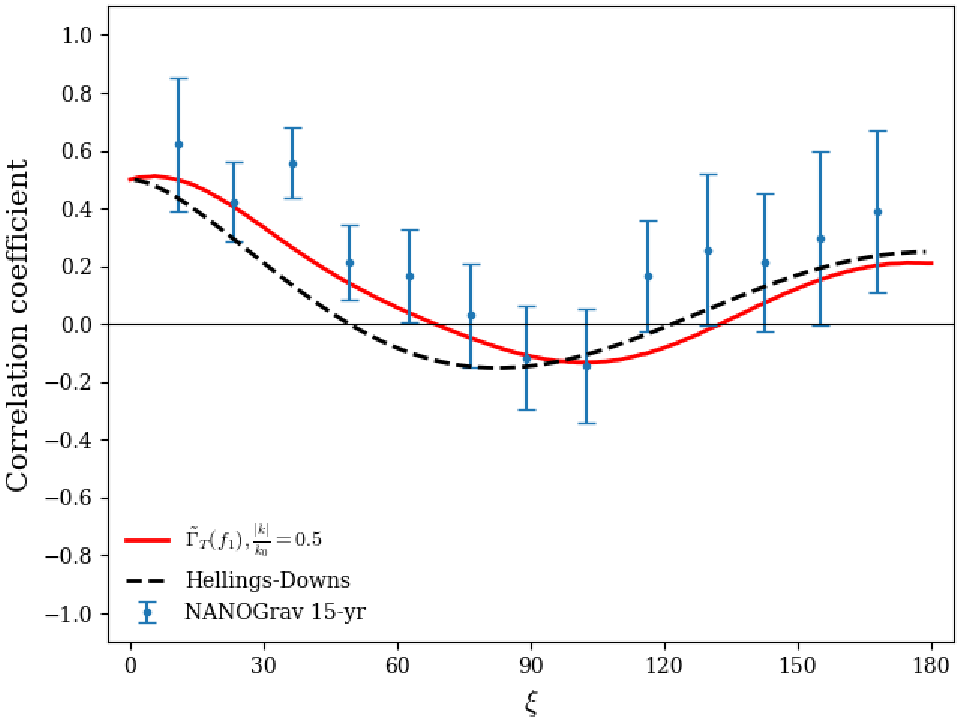
\includegraphics[width=0.8\textwidth]{fig2.pdf}
    \caption{The frequency-dependent ORF plotted as a function of $fL$. We see that for $fL$ near 1, the ORF is certainly not negligibly different from its frequency-independent value.}
    \label{fig:freq_dep}
\end{figure}
We use Monte-Carlo integration to numerically compute the frequency dependence of the effective ORF. The magnitude of $\Gamma_T(|f_{\text{min}}|)$ is significantly greater than $\Gamma_T$ with the factors of $\mathcal{E}(f, \hat{\bf \Omega})$ suppressed. If the ORF is in the regime where the Taylor expansions in the short wavelength ($fL \gg 1$) or long wavelength ($fL \ll 1$) cannot be carried out, then we must not ignore $\mathcal{E}(f, \hat{\bf \Omega})$.
\begin{figure}[h]
    \centering
    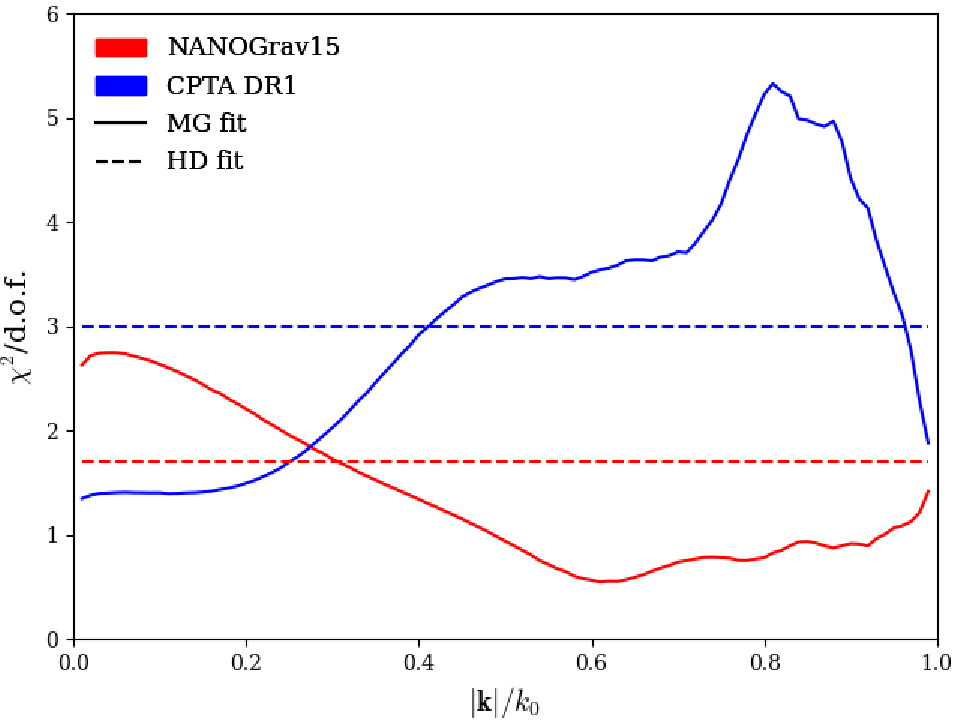
\includegraphics[width=0.6\textwidth]{fig3.pdf}
    \caption{The ORFs plotted as a function of angular separation $\xi$. The solid lines use the full expression of the ORFs, including the factors of $\mathcal{E}$. The dotted lines are frequency independent and ignore the factors of $\mathcal{E}$. The solid lines are plotted with $fL = 1$}
    \label{fig:orfs}
\end{figure}
In Fig.\ \ref{fig:orfs}, we see how differently the ORFs behave when we take into account the frequency dependence and when we ignore it. We observe that for a fixed $fL$, the ratio $|{\bf k}|/k_0$ corresponds to an increasing disparity between the frequency-dependent and -independent ORFs. For sufficiently small values of the ratio $|{\bf k}|/k_0$, e.g.\ $|{\bf k}|/k_0 \lesssim 0.1$, the frequency-dependent ORF acquires additional local extrema, namely a minimum and a maximum. This is a peculiarity that only arises when factors of $\mathcal{E}$ are taken into account. We also expect such a drastic behavior to emerge when the mass of the graviton is sufficiently high, which corresponds to the ratio according to 
\begin{equation}\label{eqn:ratio_m}
    \frac{|{\bf k}|}{k_0} = \sqrt{1 - \frac{m^2}{k_0^2}}
\end{equation}

\subsection{Graviton Mass}\label{subsec:mass}
The graviton mass is intimately connected to the behavior of the effective ORF. It appears as a ratio between the mass and the effective angular frequency, through Eq.\ \ref{eqn:ratio_m}. If observations of PTAs follow the trajectory for the best-case scenario, as detailed in Sec.\ \ref{subsec:exp_fac}, then we can only hope to observe a graviton mass given by that lower frequency bound. This corresponds to $m_g \sim 1.31\times 10^{-24} \eV$. To be clear, we are assuming that the lowest theoretical frequency that we can probe, given by the limit of Eq.\ \ref{eqn:omega} as $k\rightarrow 0$, will coincide with the lowest practical frequency that PTAs can measure, hence the ``best-case'' scenario. Going forth, this is the mass that we will take $m_g$ to be in our analysis.

The graviton mass affects all the ORFs for each polarization type, including the tensor modes. The graviton mass shows up in the exponential terms as the coefficient in front of the dot product $\sqrt{1 - (m_g/k_0)^2}\hat{\bf \Omega}\cdot \hat{\bf p}_j$ and in the massive spin-1 helicity-0 polarization vector $\epsilon_\mu^0(m_g) = \sqrt{1 / (1 - (m_g/k_0)^2)}(\sqrt{1 - (m_g/k_0)^2}, \sin\theta\cos\varphi, \sin\theta\sin\varphi, \cos\theta)$. The former appears in all of the polarization types, but the latter only appears in the vector and scalar modes in the receiving functions, further complicating their mass dependences. The analytical expressions we are integrating can be found in Ref.\ \cite{Liang:2021bct}, except the expressions we use contain $\mathcal{E}$. Interestingly, because the graviton mass only appears as a ratio $m_g / k_0$, the behavior of the ORF is only sensitive to the mass relative to the frequency. In other words, there is no significance of an ORF purely due to a graviton mass of $m_g$. The question would be, with regards to what frequency?

\section{Results}\label{sec:results}
We now present the main results of this work. Although our calculations are for observations that extend well into the future, it is instructive to compare to current data and confirm whether they are within the present standard deviations, or perhaps explain the current data better than the Hellings-Downs. We use the NANOGrav 15-year data set to obtain the angular correlations of 2,211 pairs of pulsars from a 67-pulsar array \cite{Agazie:2023}. We also use the CPTA Data Release I to manually reconstruct the binned average values from 1,596 pairs of pulsars of a 57-pulsar array \cite{Xu:2023wog}.
\begin{figure}[h]
    \centering
    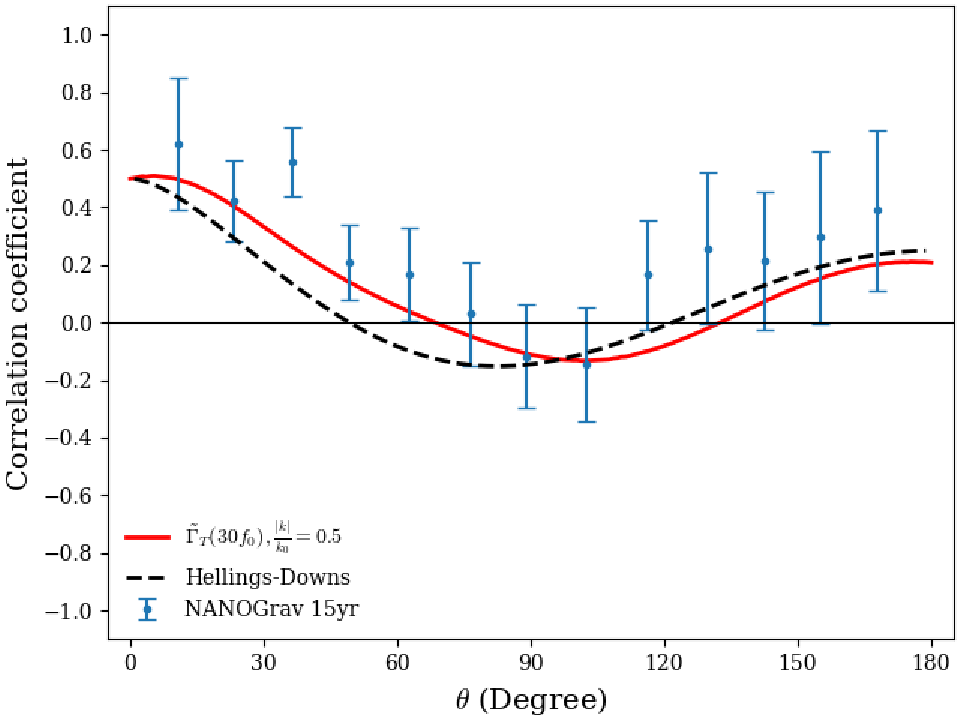
\includegraphics[width=0.5\textwidth]{fig1.pdf}
    \caption{The frequency-dependent effective overlap reduction function plotted as a function of the angular separation $\theta$ between a pair of pulsars, in red. This is plotted at the upper bound of the frequency, $\sim 30f_0$, and we set $|{\bf k}|/k_0 = 0.5$. The angular-separation–binned inter-pulsar correlations for the NANOGrav 15-year dataset are plotted in blue.}
    \label{fig:ng}
\end{figure}
We note that we do not use the frequentist optimal statistic that Ref.\ \cite{Agazie:2023} employs, which is based on methods described in Ref.\ \cite{Allen:2022ksj}, since it is crucial that the estimator is not biased towards the Hellings-Downs. We want the statistics to not assume anything about the additional polarizations so our comparison is legit. For Fig.\ \ref{fig:ng}, we used 13 bins constructed such that the mean of each bin matches the mean $\xi$'s of the CPTA data as closely as possible, since we are not able to alter the number or range of the bins in the CPTA data due to its public inaccessibility. Unfortunately, due to this complication, we compute the statistics for each binned average, rather than the correlation coefficient for each pair, since we want the statistics for the two data sets to be on equal footing.

We present Table \ref{tbl:chi}
\begin{table}[h] 
\centering
\renewcommand{\arraystretch}{1.8}
\begin{tabular}{|c|c|c|c|}
\hline
\textbf{Data} & \textbf{Fit} & \textbf{$\chi^2$} & \textbf{$\chi^2$/d.o.f.} \\
\hline
NANOGrav 15-yr & Hellings-Downs & 22.20 & 1.71 \\
\hline
NANOGrav 15-yr & Massive Gravity & 11.22 & 1.02 \\
\hline
CPTA DR1 & Hellings-Downs & 38.95 & 3.00 \\
\hline
CPTA DR1 & Massive Gravity & 16.58 & 1.51 \\
\hline
\end{tabular}
\caption{The $\chi^2$ and $\chi^2$/d.o.f.\ values for diferent fit functions for the two datasets used in this analysis. We have 13 degrees of freedom for the Hellings-Downs correlation and 11 for the massive gravity models, with 2 fit parameters: $m_g$ and $f$. }
\label{tbl:chi}
\end{table}
for the statistics in our analysis. We see that 

\begin{figure}[h]
    \centering
    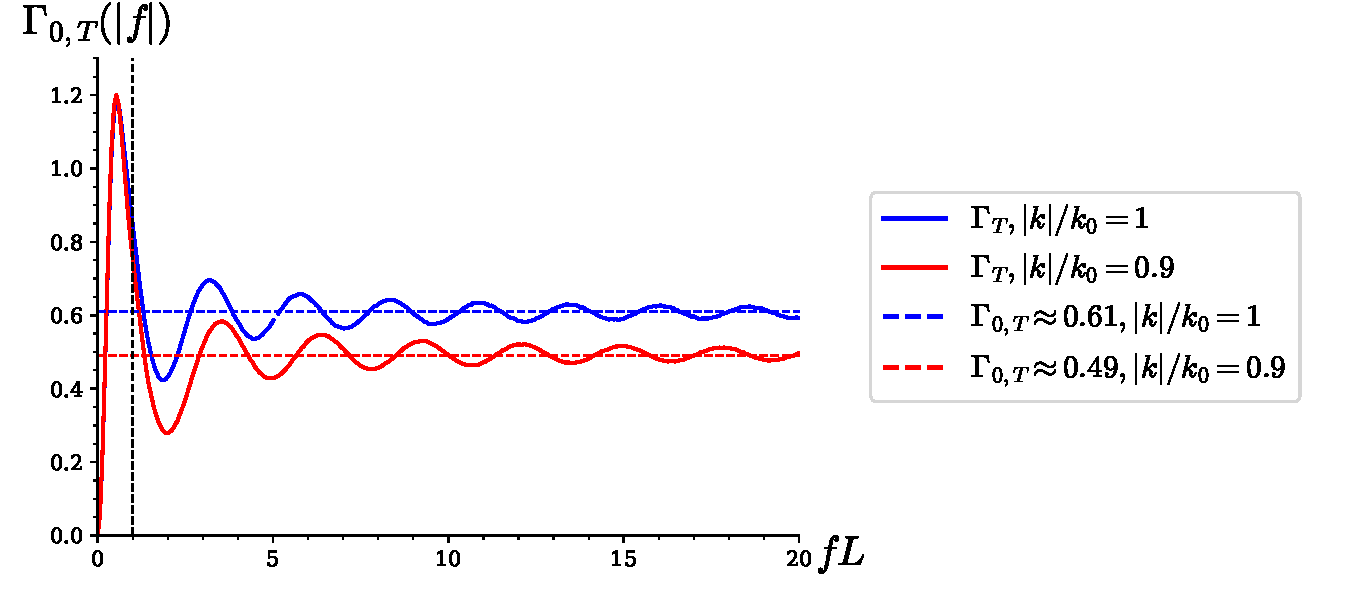
\includegraphics[width=0.5\textwidth]{fig0.pdf}
    \caption{The frequency-dependent effective overlap reduction function plotted as a function of the angular separation $\theta$ between a pair of pulsars, in red. This is plotted at the lower bound of the frequency, $f_0$, and we set $|{\bf k}|/k_0 = 0.1$. The angular–separation–binned inter-pulsar correlations for the CPTA dataset for $f_0$ are plotted in blue. The bins are chosen to match the results of Ref.\ \cite{Xu:2023wog}, since their data are not public.}
    \label{fig:cpta}
\end{figure}

\section{Discussion}\label{sec:discussion}

\vspace{3mm}
The NANOGrav 15-year data used in this paper are publicly available at NANOGrav. Source code to reproduce all of the figures and Table \ref{tbl:chi} is available in our GitHub repository.

\begin{center}
    \textbf{ACKNOWLEDGMENTS}    
\end{center}
\ \ \ We thank Murman Gurgenidze and Qiuyue Liang for useful discussions related to the paper. We also thank the organizers of the Phenomenology 2025 Symposium, for which much of this paper has been developed. C.C.\ and T.K.\ acknowledge support from the NASA Astrophysics Theory Program (ATP) Award 80NSSC22K0825 and the National Science Foundation (NSF) Astronomy and Astrophysics Research Grants (AAG) Award AST2408411.

\bibliographystyle{apsrev4-2_edited}
\bibliography{refs}

\clearpage
\end{document}
Recent detection of stochastic gravitational wave background via 15-year observation 
have further ignited interest in the gravitational wave astronomy, and its application to constrain fundamental physics, and correspondingly to better understand the nature of gravity. 
The detected PTA signal can be understood, along with the possibility of the astrophysical sources  (such as supermassive black holes) induced gravitational waves, as a signal possibly from the early universe \cite{Figueroa:2023zhu}. Actually 
relic gravitational waves promise a new window into the highest-energy events in the evolution of the universe: indeed gravitational radiation propagates {\it almost} (see below) freely throughout cosmic history, and primordial gravitational waves reflect a precise picture of the universe at their time of production in the first fractions of a second after the Big Bang.  
Detecting these gravitational waves today would open the possibility of testing physical processes at extreme energy scales far beyond what is reached by particle physics experiments and astrophysical observations \cite{Chongchitnan:2006pe}. 